\documentclass[10pt,twoside]{article}
\usepackage[utf8]{inputenc}
\usepackage{amsmath}
\usepackage{amsfonts}
\usepackage{amssymb}
\usepackage[spanish,es-noshorthands]{babel}
\usepackage[T1]{fontenc}
\usepackage{lmodern}
\usepackage{graphicx,hyperref}
\usepackage{tikz,pgf}
\usepackage{multicol}
\usepackage{subfig}
\usepackage[papersize={6.5in,8.5in},width=5.5in,height=7in]{geometry}
\usepackage{fancyhdr}
\pagestyle{fancy}
\fancyhead[LE]{
\includegraphics[height=12pt]{Images/logo-colegio.png} Aritmética $6^{\circ}$}
\fancyhead[RE]{}
\fancyhead[RO]{\textit{Germ\'an Avenda\~no Ram\'irez, Lic. U.D., M.Sc. U.N.}}
\fancyhead[LO]{}

\author{Germ\'an Avenda\~no Ram\'irez, Lic. U.D., M.Sc. U.N.}
\title{\begin{minipage}{.2\textwidth}

\includegraphics[height=1.75cm]{Images/logo-colegio.png}\end{minipage}
\begin{minipage}{.55\textwidth}
\begin{center}
Taller 06\\Adición y sustracción en $\mathbb{N}$  \\
Aritmética $6^{\circ}$
\end{center}
\end{minipage}\hfill
\begin{minipage}{.2\textwidth}

\includegraphics[height=1.75cm]{Images/logo-sed.png} 
\end{minipage}}
\date{}
\begin{document}
\maketitle
Nombre: \hrulefill Curso: \underline{\hspace*{44pt}} Fecha: \underline{\hspace*{2.5cm}}
\section*{Continuaci\'on gu\'ia 5}
\subsection*{Actividad 1}
En tu cuaderno:
\begin{enumerate}
\item ¿Para qué valor de $x$ se cumple que:
\begin{enumerate}
\begin{multicols}{2}
\item $x+12=17$?
\item $8+x=20$?
\item $7+x=7$?
\item $x+11=11$?
\item $(5+x)+3=10$?
\item $13+17=x$?
\end{multicols}
\end{enumerate}
\item Un agricultor recogió la cosecha de papa en una semana así: el lunes 23 bultos, el martes 36 bultos, el miércoles 17 bultos, el jueves 19 bultos, el viernes 18 bultos y el sábado 21 bultos. ¿Cuántos bultos de papa recogió en total?

\begin{minipage}{0.45\textwidth}
\item Completa el siguiente cuadro en tu cuaderno con los números naturales
correspondientes.
\end{minipage}\hfill
\begin{minipage}{.45\textwidth}
\begin{tabular}{|c|c|c|c|}
\hline 
\multicolumn{3}{|c|}{SUMANDOS} & TOTAL \\ 
\hline 
8 & 2 & 0 &  \\ 
\hline 
9 &  & 1 & 20 \\ 
\hline 
0 &  & 5 & 12 \\ 
\hline 
 & 7 & 6 & 18 \\ 
\hline 
\end{tabular} 
\end{minipage}

\begin{minipage}{.45\textwidth}
\item Completa el siguiente cuadro en tu cuaderno de tal forma que en la diagonal
aparezcan las adiciones correspondientes.
\end{minipage}\hfill
\begin{minipage}{.45\textwidth}
\begin{tabular}{ccccc}
 & $a$ & $b$ & $c$ & $a+b+c$ \\ 
\cline{2-5} 
a & \vline \hfill 5 \hfill \vline & 8 \hfill \vline & 3 \hfill \vline & \hfill \vline   \\ \cline{2-5}
b & \vline \hfill 8 \hfill \vline & 16 \hfill \vline & \hfill \vline & \\ \cline{2-4}
c & \vline \hfill 3 \hfill \vline & \hfill \vline & 6 \hfill \vline & \\ \cline{2-4}
$a+b+c$ &  \vline \hfill \hspace*{10pt} \hfill \vline & & \\ \cline{2-2}
\end{tabular} 
\end{minipage}
\end{enumerate}
\section*{Sustracci\'on de n\'umeros naturales}
\subsection*{Actividad 2}
Supón que en la finca de tu vecino se recogieron ayer 9 bultos de naranja y se
llevaron a la ciudad 7 de ellos para venderlos. ¿Cuántos bultos de naranja le
quedaron al vecino?

Responde:
\begin{itemize}
\item ¿Cuántos bultos de naranja tenía inicialmente?
\item ¿Cuántos bultos de naranja vendió?
\item ¿Cuántos bultos le quedan en la finca?
\item Si sumas el número de bultos que vendió con el número de bultos que le
    quedan en la finca, ¿cuántos bultos obtiene en total?
\item ¿Cuanto le falta a 7 para ser igual a 9?
\item ¿Cuánto le falta a 2 para ser igual a 7?

Lo anterior se puede expresar así: 
\begin{align*}
7 + 2 &= 9\\
2+7&=9\\
\mbox{Si } 2+7=9, \mbox{ entonces }\qquad 9-2&=7\\
9-7&=2 
\end{align*}
\item ¿Qué clase de número es el 7?
\end{itemize}
Analiza la siguiente conclusión:

La operación inversa de la adición de números naturales es la SUSTRACCIÓN,
luego si $a + b = c$, entonces $c - a = b$. Al número natural $c$ se llama MINUENDO,
al natural $a$ SUSTRAENDO y al natural $b$ DIFERENCIA.

En el caso anterior:
\[
\begin{array}{ccccc}
9 & - & 2 & = & 7 \\
Minuendo &  & Sustraendo &  & Diferencia
\end{array}
\] 
El signo de la SUSTRACCIÓN: -- (Se llama menos)
\subsection*{Actividad 3}
Nos reunimos en parejas y realizamos los siguientes ejercicios:
\begin{enumerate}
\item Si $a$, $b$, $c$ son números naturales definidos así: $a = 8$; $b = 15$; $c = 3$; realizamos las siguientes sustracciones:
\begin{multicols}{2}
\begin{enumerate}
\item $a-c$
\item $b-a$
\item $b-c$
\item $a-b$
\end{enumerate}
\end{multicols}
¿Algún problema?
\item ¿Cómo debe ser el minuendo comparado con el sustraendo para poder efectuar la
diferencia?
\item ?`Cu\'anto le falta al natural 10 para ser igual al natural 17?
\item Realicemos las siguientes operaciones:
\begin{enumerate}\begin{multicols}{2}
 \item 15-8= \item 13-7= \item 14-9= \item 16-6= \item 8-15= \item 7-13= \item 9-14= \item 6-16=
\end{multicols}
\end{enumerate}
\begin{itemize}
 \item ?`Qu\'e conclusi\'on podemos sacar de este ejercicio?
\item ?`Es la sustracci\'on una operaci\'on que cumple la propiedad conmutativa?
\end{itemize}
\item Realicemos las siguientes operaciones
\begin{enumerate}
 \item $9-(4-3)=9-1=8$
\begin{multicols}{2}
 \item $18-(8-6)=$? \item $14-(7-2)=$?
\end{multicols}\end{enumerate}
\item Realicemos las siguientes operaciones:
\begin{enumerate}\begin{multicols}{2}
 \item $(9-4)-3=$?
\item $(18-8)-6=$?
\item $(14-7)-2=$?
\end{multicols}
\end{enumerate}
\begin{itemize}
 \item Comparemos los resultados de los ejercicios 5 y 6.
\item ?`Qu\'e conclusi\'on podemos sacar?
\item ?`Cumple la sustracci\'on con la propiedad asociativa?
\end{itemize}
\item Realicemos las siguientes sustracciones:
\begin{itemize}\begin{multicols}{2}
\item \fbox{$6-0$} \item \fbox{$7-0$} \item \fbox{$0-6$} \item \fbox{$0-7$}
\end{multicols}\end{itemize}
?`Qu\'e podemos concluir de la diferencia con respecto a la propiedad modulativa?
\item Analicemos la siguiente conclusi\'on:\\
La diferencia entre n\'umeros naturales \textbf{no cumple} con las propiedades clausurativa, conmutativa, asociativa y modulativa.
\end{enumerate}
\subsection*{Actividad 4}
Trabajo individual:\\
Resuelve los siguientes problemas:
\begin{enumerate}
 \item Juan va al mercado y compra un kilo de papa que le cuesta \$1200, un kilo de carne \$10000, una libra de arroz por \$1250 y fruta por \$5500. Si llevaba en su cartera \$25000. ?`Cu\'anto dinero le sobr\'o?
\item En una escuela hay matriculados 25 alumnos en primer grado, 36 en segundo grado, 12 en tercero, 24 en cuarto grado. Si la escuela tiene un total 132 alumnos en los cinco grados, ?`cu\'antos alumnos hay en quinto grado?
\item Nos reunimos en grupos de m\'aximo 3 personas y comparamos las respuestas con los anteriores ejercicios. Corregimos los errores.
\end{enumerate}
\subsection*{ACTIVIDAD 5 (Trabajo individual)}
Colocar en cada c\'irculo uno de los n\'umeros de 1 a 12. No se puede repetir ninguno. La suma de los n\'umeros que resulten en cada lado del tri\'angulo debe ser la misma.
\begin{center}
 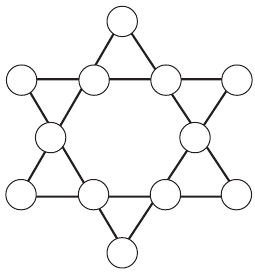
\includegraphics{Images/estrella.png}
 % estrella.png: 255x272 pixel, 96dpi, 6.75x7.20 cm, bb=0 0 191 204
\end{center}
\end{document}
